% !TeX spellcheck = en_US

\chapter{Basis}
\label{chap:basis}
In this chapter, the common terms will be explained.
\section{Cloud Computing and Cloud application} \label{sec:cloud}

\subsection{Definitions}
Unfortunately, generally accepted definition of cloud computing that describes all possible situations doesn't exist. 
But in the scientific community, the definition put forward by \textbf{N}ational \textbf{I}nstitute of \textbf{S}tandards and \textbf{T}echnology (NIST) is commonly used. 
This definition appropriately describes the concept of cloud computing used in this paper, and therefore this definition will be used and presented below.
\begin{definition}[Cloud computing]
	\label{def:nist}
$Cloud$ $computing$ is a model for enabling ubiquitous, convenient, on-demand network access to a shared
pool of configurable computing resources (e.g., networks, servers, storage, applications, and services) that
can be rapidly provisioned and released with minimal management effort or service provider interaction. \cite*{nist}
\end{definition}
Also, the are no generally accepted definitions of cloud application, but it can be obtained from the definition of cloud computing.
\begin{definition}[Cloud application] 
	\label{def:capp}
	A $Cloud$ $application$ is an application that is executed according to a cloud computing model. \cite*{cloudapp}
\end{definition} 
In addition, a short definition of cloud system will be provided.
\begin{definition}[Cloud system] 
	\label{def:csys}
Composite cloud applications which consists of multiple small application will ba called a $cloud$ $system$.
\end{definition} 
%\subsubsection{Sides}
An owner of physical platform, where cloud computing takes place is called a $provider$.
An owner of cloud application, renting a provider's platform is called a $user$.
\subsubsection*{Service models}\label{def:servmod}
NIST distinguishes between three types of service models.
\begin{itemize}
	\item Software as a Service (SaaS). 
	The capability provided to the consumer is to use the provider’s applications running on a cloud infrastructure. 
	The applications are accessible from various client devices through either a thin client interface, such as a web browser (e.g., web-based email), or a program interface. 
	The consumer does not manage or control the underlying cloud infrastructure including network, servers, operating systems, storage, or even individual application capabilities, with the possible exception of limited userspecific application configuration settings.
	\item Platform as a Service (PaaS). 
	The capability provided to the consumer is to deploy onto the cloud infrastructure consumer-created or acquired applications created using programming languages, libraries, services, and tools supported by the provider.
	The consumer does not manage or control the underlying cloud infrastructure including network, servers, operating systems, or storage, but has control over the deployed applications and possibly configuration settings for the application-hosting environment.
	\item Infrastructure as a Service (IaaS).
	The capability provided to the consumer is to provision processing, storage, networks, and other fundamental computing resources where the
	consumer is able to deploy and run arbitrary software, which can include operating systems and applications.
	The consumer does not manage or control the underlying cloud infrastructure but has control over operating systems, storage, and deployed applications; and possibly limited control of select networking components (e.g., host firewalls).
\end{itemize}

\subsubsection*{Deployment models}
Similarly, NIST distinguishes between four types of deployment models.
\begin{itemize}
	\item Private cloud. 
	The cloud infrastructure is provisioned for exclusive use by a single organization comprising multiple consumers (e.g., business units). It may be owned, managed, and operated by the organization, a third party, or some combination of them, and it may exist on or off premises.
\item Community cloud.
	The cloud infrastructure is provisioned for exclusive use by a specific community of consumers from organizations that have shared concerns (e.g., mission, security requirements, policy, and compliance considerations).
	It may be owned, managed, and operated by one or more of the organizations in the community, a third party, or some combination of them, and it may exist on or off premises.
\item Public cloud.
	The cloud infrastructure is provisioned for open use by the general public. 
	It may be owned, managed, and operated by a business, academic, or government organization, or some combination of them.
	It exists on the premises of the cloud provider.
\item Hybrid cloud. 
	The cloud infrastructure is a composition of two or more distinct cloud infrastructures (private, community, or public) that remain unique entities, but are bound together by standardized or proprietary technology that enables data and application portability (e.g., cloud bursting for load balancing between clouds). 
\end{itemize}

\subsection{Usage}
Now cloud computing and application can be found everywhere, and they number constantly grows. \cite*{cloud_stat}
They are used for test and development, big data analyses, file storage and so on.
Cloud computing allows using resources effectively, to distribute the load to a system from several physical servers and to shift the maintenance to the providers. 
If service uses a single one physical server and this server will be disabled, then entire service will be completely unavailable too.
But if cloud application uses a hundred of physical servers, then disabling of one will not carry such serious consequences.
In addition, a user doesn't need to maintain a team of administrators for the event of various problems.\\
Usually, a user doesn't have direct access to the infrastructure (servers and operating systems), he uses only provided Application Programming Interface (API).
An API provides a set of methods to communicate with provider's infrastructure. 
Each provider defines his own set of methods, depending on his area of specialization. 
On the one hand, this specialization makes easier to work with the provider, on the other hand, it becomes more difficult to redeploy an application to another provider.

\section{Topology and Orchestration Specification for Cloud	Applications (TOSCA)} \label{sec:tosca}
\subsection*{Definition}
The OASIS \cite{oasis} Topology and Orchestration Specification for Cloud Applications (\gls{tosca}) standard provides a new way to enable portable automated deployment and management of a cloud applications.
\gls{tosca} describes the structure of applications as topology containing their components and relationships between them.
%Plans capture management tasks by orchestrating management operations exposed by the components. \cite*{INBOOK-2014-01}
\gls{tosca} application is a cloud application described according to TOSCA standard.
\gls{tosca} can be used not only for describing all stages of a cloud application life-cycle but also serve as a layer between the cloud application and provider's API, allowing to implement a single application suitable for working with different providers. 
\subsection*{Structure}
TOSCA specification provides a language to describe service components (described in section \nameref{def:servmod}) and relationships between them using a Service Topology. 
In additional it defines the management procedures which create or modify services using orchestration processes.\\
Descriptions of the \gls{tosca}'s main components used in this work is provided below.
\begin{itemize}
\item $Service$ $Template$ is the main component in \gls{tosca} structure. 
It contains an information about structure (Topology Template) and interfaces (Plans) of the cloud application.
\item A $Plan$ provides an interface to manage cloud application.
These components combine management capabilities to create higher-level management tasks, which can then be executed fully automated to deploy, configure, manage, and operate the application.
Plans are started by an external message and call management operations of the nodes in the topology.
\item $Topology$ $Template$ describes the topology of cloud application, instantiating nodes (Node Templates) and relations between them (Relationship Templates).
\item $Node$ $Template$ specifies the occurrence of a Node Type as a component of a service.
\item $Node$ $Type$ defines the properties of such a component and the operations available to manipulate the component.
\item $Relationship$ $Template$ specifies the occurrence of a Relationship Type as a relationship between Node Templates in a Topology Template. 
	The Relationship Template indicates the elements it connects and the direction of the relationship by defining one source and one target element (in further Source Element and Target Element).
\item $Relationship$ $Type$ defines the semantics and any properties of the relationship. \label{subs:reltype}
\item $Artifact$ represents the content needed for a management such as executables (e.g. a script, an executable program, an image), a configuration file or data file, or something that might be needed for other executables (e.g. libraries).
	TOSCA distinguishes two kinds of artifacts: Implementation Artifacts and Deployment Artifacts.
\item $Implementation$ $Artifact$ represents the executable of an operation described by Node Type.
\item $Deployment$ $Artifact$ represents the executable for materializing instances of a node.
\item $Artifact$ $Type$ describes a common type of an artifact: python script, installation package and so on.
\item $Artifact$ $Templates$ represents information about the artifact. 
	Artifact location and other attendant data are stored here.
\item $Node$ $Type$ $Implementation$ defines the artifacts needed for implementing the corresponding Node Type.
For example, if Node Type contains $deploy$ and $shutdown$ operations, then Node Type Implementation can contain two Implementation Artifacts with scripts for these operations and one Deployment Artifact with data needed for the deployment.
\end{itemize}
Types and Templates defining a TOSCA application are stored in definition documents, which have the XML structure.\\
\subsection*{Usage}
The combination of topology and orchestration in a Service Template defines what is needed to be preserved across deployments in different environments to enable interoperable deployment of cloud services and their management throughout the complete lifecycle (e.g. scaling, patching, monitoring, etc.).
This is useful when an application is ported to alternative cloud environments. \cite{TOSCA-v1.0_book} \\

\subsection{CSAR} \label{sec:csar}
A \gls{csar} is used to store the TOSCA application.
It is a ZIP-file with ".csar" extension that contains all the data needed for instantiation and management of TOSCA application.
These include definition documents, artifacts and so on.
In this form, a TOSCA application can be processed by a TOSCA runtime environment.
\subsubsection*{Structure}
The root folder must contain a "Definitions" and a "\gls{tosca}-Metadata" folders.
The "Definitions" folder contains definition documents and one of them must define Service Template.
The "\gls{tosca}-Metadata" folder must contain TOSCA metadata in form of file with the "TOSCA.meta" name.
This metafile consists of name/value pairs. 
One line for each pair. 
The first set of pairs describes CSAR itself (TOSCA version, CSAR version, creator and so on). 
All other pairs represent metadata of files in the CSAR. 
The metadata is used by TOSCA runtime environment to correctly proceed given files.

\subsubsection*{Terms}
Input \gls{csar} is a \gls{csar}, which can contain external references and will be processed by the framework.\\
Output CSAR is a CSAR, which was processed by the framework and doesn't contain external references (at least those that are implemented in the framework).

\section{OpenTOSCA} \label{sec:opentosca}
OpenTOSCA provides an open source ecosystem for \gls{tosca} applications. 
The OpenTOSCA ecosystem consists out of three parts: \cite*{OpenTOSCA}
\begin{itemize}
	\item OpenTOSCA \textbf{Container}, a \gls{tosca} runtime environment
	\item \textbf{Winery} \label{tool:winery}, a graphical modelling TOSCA tool.
	\item \textbf{Vinothek}, a self-service portal for the applications available in the container
\end{itemize}
The runtime environment ant Winery will be provided in more details. 
\subsection*{Runtime environment}
The runtime enables fully automated plan-based deployment and management of applications in the CSAR format. 
First, the CSAR is unpacked and the files are put into the Files store.
Then, the TOSCA definitions documents are loaded, resolved, validated, and processed by the Control component, which calls the Implementation Artifact Engine and the Plan Engine.
The Implementation Artifact Engine deploys the referenced Implementation Artifacts and stores their endpoints in the Endpoints database. 
Finally, the Plan Engine binds and deploys the application’s management plans.
The endpoints of the management plans are stored in the Plans database.
\cite{INPROC-2013-45}
\subsection*{Winery}\label{subs:wine}
Winery works under the Tomcat runtime and therefore visual interface is available in browser, example in figure \ref{fig:winery_gui}.
Winery provides a complete set of functions for creating, editing and deleting all elements of the TOSCA topology. 
An example of TOSCA topology is presented on figure \ref{fig:winery_source}.
\begin{figure}[ht]   
	\centering
	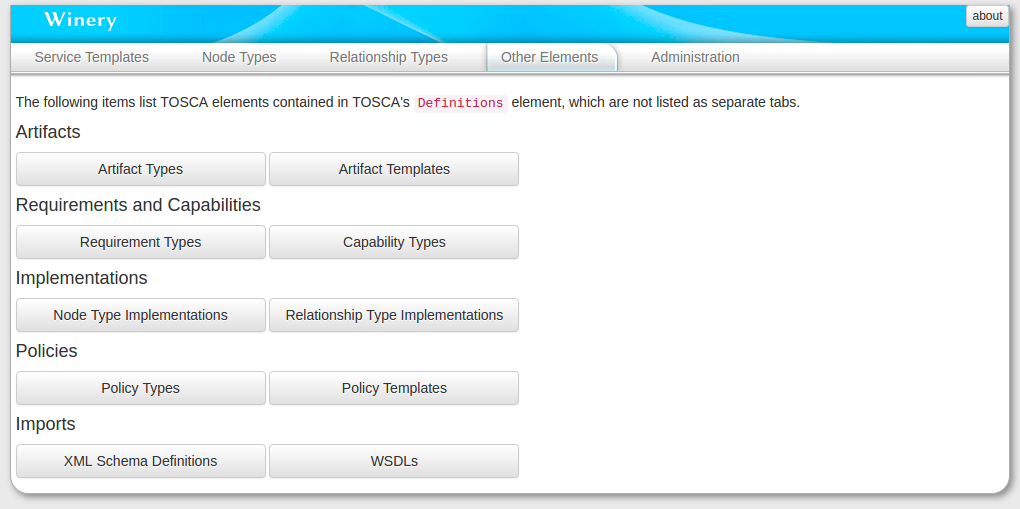
\includegraphics[width=0.7\textwidth]{Screenshot_winery_gui.png}
	\caption{Visual interface for $Winery$.}
	\label{fig:winery_gui}
\end{figure}
\begin{figure}[ht]   
\centering
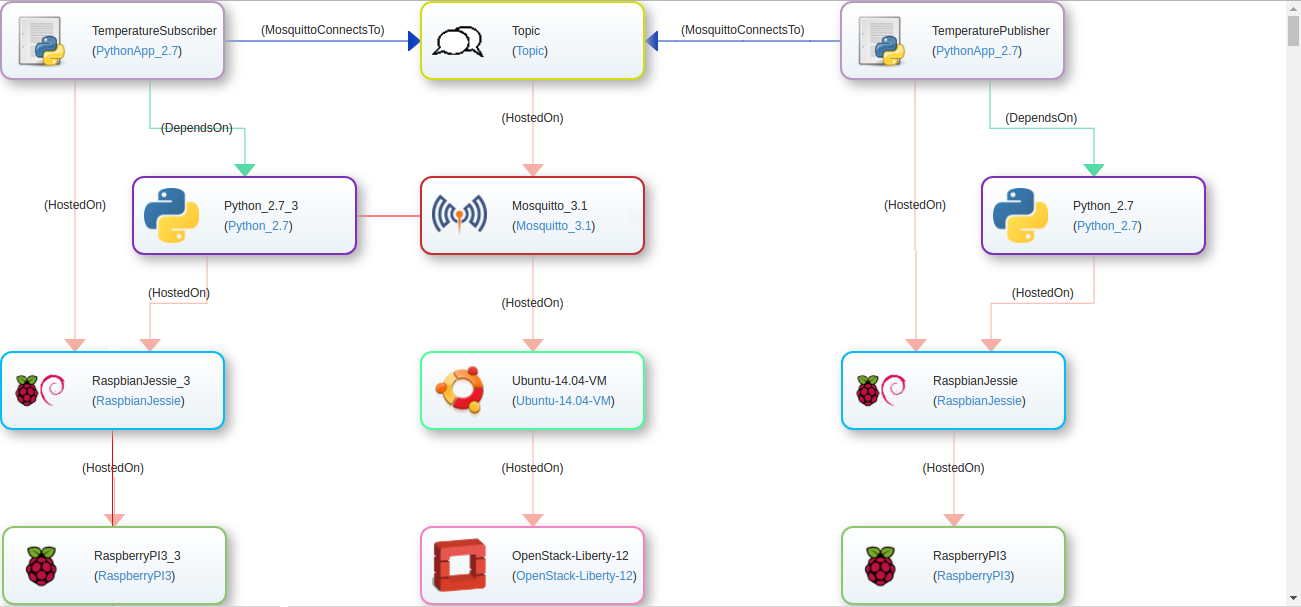
\includegraphics[width=0.7\textwidth]{Screenshot_winery_source.png}
\caption{TOSCA topology presented by $Winery$.}
\label{fig:winery_source}
\end{figure}


\section{Package management} \label{sec:pm}
This section will describe the package management process and basic concepts from this area.
\subsection*{Package managers}
Package Manager is a set of software tools that automate the process of installing, updating, configuring and removing of computer programs.
A package can describe and contain not only a whole program, but also a certain component of a large application, hereinafter both will be referred as program components.
Package managers are used to manage the database of packages, their dependencies and versions, to prevent erroneous installation of programs and missing dependencies.
\subsection*{Packages}
A package is usually an archive containing both data for installation of the program component and a set of metadata like name, function, version, producer and dependencies.
\subsection*{Dynamic libraries}
Computer systems which rely on dynamic library linking, share executable libraries of machine instructions across packages and applications. 
In these systems, complex relationships between different packages requiring different versions of libraries results in a challenge colloquially known as "dependency hell".
Good package management is vital on these systems.
\subsection*{Repository}
To give users more control over the kinds of software that they are allowing to be installed on their system, software is often downloaded from a number of software repositories.
By default in Unix systems a package manager uses official repositories appropriate for the operating system and the device architecture, but the user can also additional repositories, like third-party repositories or repositories for another architecture.
\subsection*{Dependencies} \label{subs:dep}
Package managers distinguish between two types of dependencies: $required$ and $preRequired$.
Dependency $package1$ $required$ $package2$ indicates that $package2$ must be installed for proper operation of $package1$.
Dependency $package1$ $preRequired$ $package2$ indicates that $package2$ must be installed for proper installation of $package1$.
An example of obtaining a dependency list is shown in listing \ref{lst:dep}.
\begin{lstlisting}[caption={Example of using $apt$-$cache$ to obtain dependency list for package python}\label{lst:dep},captionpos=t] 
user@user:~$ apt-cache depends python
python
PreDepends: python-minimal
Depends: python2.7
Depends: libpython-stdlib
Conflicts: <python-central>
Breaks: update-manager-core
Suggests: python-doc
Suggests: python-tk
Replaces: python-dev
\end{lstlisting}
\subsection*{Dependency tree}
In the example above $package2$ is needed for $package1$, but $package2$ itself can require additional packages.
A structure describing all needed packages and dependencies between them for given root-package is called a dependency tree. 
Dependency type $required$ leads to the presence of cycles in dependency tree, which differs them from normal tree graph structures.

\section{Package management automation}
To automate the package management, various environment are used. 
Those environments will be described, which will be used in the framework.
\subsection{Bash} \label{lang:bash}
Bash is a Unix shell and command language written as a free software.
Bash is a command processor that typically runs in a text window, where the user types commands that cause actions.
Bash can also read and execute commands from a file, called a script. \cite{bash}
\subsection{Ansible} \label{lang:ansible}
Ansible is an open-source automation engine that automates software provisioning, configuration management, and application deployment.
As with most configuration management software, Ansible has two types of servers: controlling machines and nodes.
First, there is a single controlling machine which is where orchestration begins.
Nodes are managed by a controlling machine over SSH.
The controlling machine describes the location of nodes through its inventory.
Ansible playbooks express configurations, deployment, and orchestration in Ansible.
The playbook format is YAML. 
Each playbook maps a group of hosts to a set of roles.
Each role is represented by calls to Ansible tasks.
 \cite{ansible} 
